\chapter{Work Process}

Our team consists of four members. We started early with reading documentations about Redis and searched for code snippets to see how the magic is done. After we established a basic understanding we used our newly won knowledge to define a general data model which is detailed described in a later section. Based on this model we followed up different paths of implementation. Each path ended in a successful and usable solution. While working on different ways we shared our experiences, so that everyone is able to understand how things were managed. We learned from each other.

\section{Scenario}

As an example scenario, we will use network data stored in Redis and queried over various use cases. Storing and analyzing network data is important for security. By capturing the network flow we can look into two different granularities, the flow level and the packet level. In this scenario we will look at the packet level.

\subsection{Queries}
In order to analyze the network data we had been given various queries which should be implemented with redis. These are the queries we had to solve:
\begin{itemize}
	\item Query 1:
Retrieve all active connections at a certain point of time. Whereas active means that a package existed within the last second

\item Query 2:
Retrieve the overall data volume per minute for all connections between IP a.b.c.d and IP w.x.y.z

\item Query 3:
Retrieve all hosts that had connections to IP a.b.c.d on the HTTP port.

\item Query 4:
Retrieve all hosts that had incoming connections on well-known ports

\item Query 5:
Retrieve all packages that contain the byte sequence 0x35 0xAF 0xF8

\item Query 6:
Retrieve all hosts that had connections to outside hosts

\end{itemize}

\section{The Plan}

With the given scenario it was planned to have two different entities. One called “package” holding all for the queries needed attributes like “timestamp” or “source address” and the second called “data” for storing the raw data of the ethernet packages. Having two entities requires an association connecting these two objects. But first the objects must be created. Redis provides a suitable data type for doing so: Hashes. A hash consists of a several key-value fields while a prefixed key identifies a single hash. Addressing this key means getting the whole hash with all its fields. To search for specific hashes incremental numerical indexes should be generated. The same goes for each field of the hash. Additional to a field key a numerical index should be defined. This way those fields’ values of several hashes can be aggregated in a range. 

  \begin{figure}[htb!]
	\centerline{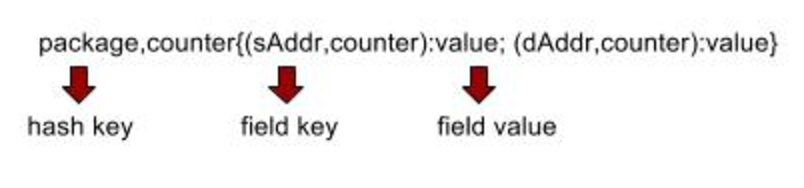
\includegraphics[width=0.8\textwidth]{resources/plan.png}}
\end{figure}

Converting the pseudo code into a valid Redis command it would look like this:

redis.hmset((‘package’,counter),{‘sAddr’,counter: sAddr})

Each field inside a single hash is an attribute of an ethernet packet. These attributes are labeled the following:
\begin{itemize}
	\item timestamp as Integer
	\item sourceAdress as Long
	\item sourceAdressPrivate as Boolean
	\item sourcePort as Integer
\item 	sourcePortWellKnown as Boolean
\item 	destinationAdress as Long
\item 	destinationAdressPrivate as Boolean
\item 	destinationPort as Integer
\item 	destinationPortWellKnown as Boolean
\end{itemize}

For the “data” entity in contrast simple Strings are applied. These strings should store the attributes “data” and “data.length”: redis.set(payload, data) and redis.set(payloadLength, data.length)
Because Redis provides commands to get any key and its value, needing an association between the “data” and “package” is left out. Instead each entity could be accessed directly. When the need to address both entities comes up, multiple commands can be combined to do so. 

All data should be stored persistent and therefore written onto disk immediately. In order to achieve this the AOF mechanism should be implemented. 

The appealed indexes are kind of pre-processing. Further pre-processing is necessary regarding to check whether a source or a destination IP is private or not. The same is valid if a port is well-known. A port is well-known when its port number is lower than 1024. And a port is a Http-port when its number is 80. Private IPs vary from 10.*.*.* over 172.[16-32].*.* to 192.168.*.*. The only planned post-processing should contain the summing of the data volume per minute. 
